 
\documentclass[xcolor=svgnames]{beamer}
%
\usepackage[italian]{babel}

\usetheme{Singapore}
\setbeamertemplate{navigation symbols}{}
\setbeamertemplate{footline}[frame number]

%
\setbeamercolor{block body}{bg=AliceBlue}

\usepackage[all]{xy}
\usepackage{accents}
\usepackage{amsmath,amssymb}
\usepackage{array}
\usepackage{bibentry}
\usepackage{bm}
\usepackage{cancel}
\usepackage{comment}
\usepackage{etex}
\usepackage{macros}
\usepackage{mathscinet}
\usepackage{mathtools}
\usepackage{rotating}
\usepackage{tikz}

\hypersetup{
    colorlinks=true,
    linkcolor=blue,
    filecolor=magenta,      
    urlcolor=cyan
    }
\renewcommand{\newblock}{\relax} %% ??????????

%
%% Gianni macros
%

\DeclareMathOperator{\M}{\mathcal M}
\DeclareMathOperator{\eDeriv}{D_{\text{e}}}
\DeclareMathOperator{\grad}{grad}
\DeclareMathOperator{\mDeriv}{D_{\text{m}}}

\newcommand{\Bspaceat}[1]{B_{#1}}
\newcommand{\Bspace}[1]{B_{#1}}
\newcommand{\Ccs}[1]{C_0\left(#1\right)}
\newcommand{\Cexp}[1]{C_0^{(\cosh-1)}\left(#1\right)}
\newcommand{\Cinfcs}[1]{C_0^\infty\left(#1\right)}
\newcommand{\Cinfp}[1]{C_{\mathrm{p}}^\infty\left(#1\right)}
\newcommand{\Derivby}[1]{\frac{\Deriv}{d#1}}
\newcommand{\Lexp}[1]{L^{(\cosh-1)}\left(#1\right)}
\newcommand{\LlogL}[1]{L^{(\cosh-1)_*}\left(#1\right)}
\newcommand{\TMaxexp}{\operatorname{T}\Maxexp}
\newcommand{\WCexp}[1]{C_0^{1,(\cosh-1)}\left( #1 \right)}
\newcommand{\Wexp}[1]{W^{1,(\cosh-1)}\left(#1\right)}
\newcommand{\WlogL}[1]{W^{1,(\cosh-1)_*}\left(#1\right)}
\newcommand{\bgamma}{{\bm \gamma}}
\newcommand{\bnabla}{{\bm\nabla}}
\newcommand{\condexpectat}[3]{{\Expectation}_{#1}\left[#2 \middle| #3\right]}
\newcommand{\displacement}{\operatorname{\mathbb S}}
\newcommand{\eBspace}[1]{B_{#1}}
\newcommand{\eDerivby}[1]{\frac{\eDeriv}{d#1}}
\newcommand{\ehessianat}[2]{\prescript{e}{}\Hessian_{#1}{#2}}
\newcommand{\expbundle}{S\Maxexp}
\newcommand{\fullbundleat}[1]{\prescript{1}{}S^1\maxexpat{#1}}
\newcommand{\gaussdensity}{\gamma}
\newcommand{\gaussint}[2]{\int{#1} \gaussdensity(#2) \ d#2 \ }
\newcommand{\hullof}[1]{\operatorname{hull}\left(#1\right)}
\newcommand{\mDerivby}[1]{\frac{\mDeriv}{d#1}}
\newcommand{\maxmix}[1]{\prescript{*}{}{\Maxexp\left(#1\right)}}
\newcommand{\mhessianat}[2]{\prescript{m}{}\Hessian_{#1}{#2}}
\newcommand{\mixbundleat}[1]{\prescript{*}{}S\maxexpat{#1}}
\newcommand{\mixbundle}{\prescript{*}{}S\Maxexp}
\newcommand{\mixfiberat}[2]{{}^*S_{#1}\maxexpat{#2}}
\newcommand{\model}{\mathcal M}
\newcommand{\opensimplexon}[1]{\mathcal P_>\left(#1\right)}
\newcommand{\preBspaceat}[1]{\prescript{*}{}B_{#1}}
\newcommand{\preBspace}[1]{\prescript{*}{}B_{#1}}
\newcommand{\rosso}[1]{\textcolor{red}{#1}}
\newcommand{\sdomainat}[1]{\sdomain_{#1}}
\newcommand{\sdomain}{\mathcal S}
\newcommand{\simplexon}[1]{\mathcal P\left(#1\right)}
\newcommand{\tensorat}[3]{\prescript{#1}{}S^{#2}\maxexpat{#3}}

\renewcommand{\emph}{\rosso}
\renewcommand{\transport}[2]{{\mathbb U} _ {#1} ^ {#2}}

%
%% end Gianni's macros
%

\title{\it Intelligenza artificiale, apprendimento automatico, matematica, antropologia}

\author[G Pistone]{\bf Giovanni Pistone}

\institute[CCA]{
\includegraphics[height=4em]{pictures/deCastro-logo.pdf} \quad 
\includegraphics[height=4em]{pictures/logo Nuovo SEFIR con URL.png}}

\date{28 marzo 2023}

\begin{document} 
% 
\begin{frame}\frametitle{Un passo insieme onlus - Il salotto delle idee. Be curious.}  

\titlepage

\tiny 
web-page: \url{www.giannidiorestino.it} 

e-mail: \url{giovanni.pistone@carloalberto.org}

orcidID: 0000-0003-2841-788X

L'autore ringrazia De Castro Statistics e Nuovo SEFIR 

\nobibliography{tutto}%

\bibliographystyle{plain}

\end{frame}

\begin{frame}[plain]\tiny\frametitle{Sommario}
 Con intelligenza artificiale intendiamo oggi una collezione molto varia di tecnologie che vanno dal controllo automatico all’apprendimento automatico. In particolare l’apprendimento automatico ha avuto, molto recentemente, alcuni successi spettacolari che ora sono disponibili in applicazioni di uso di massa. Questi prodotti di successo si applicano al trattamento delle immagini, della lingua parlata, dei testi scritti. La caratteristica fondamentale di questi sistemi, che li distingue da quelli di controllo automatico, è che non sono completamente preprogrammati ma includono un sistema di apprendimento. Questo sistema di apprendimento si basa su almeno tre innovazioni metodologiche molto recenti. Queste sono le reti neurali, la sostituzione di regole sintattiche con regole semantiche, e l’uso sistematico di alte quantità di memoria. La gran parte della presentazione è dedicata ad illustrare queste tre metodologie. Concludo poi criticando le iperboli correnti secondo le quali saremmo di fronte ad una rivoluzione antropologica dovuta alla virtualizzazione. Sostengo, in linea con alcune analisi filosofiche, che siamo di fronte ad un ulteriore passo del caratteristico uso umano di dotarsi di un sistema di ritenzione della memoria sociale costituito sopratutto di utensili. Questi argomenti sono frutto dell’attività di ricerca svolta nell’ambito dell’associazione Nuovo SEFIR www.nuovo-sefir.it e della collaborazione con la filosofa Francesca dell’Orto.   
\end{frame}

\begin{frame}[plain]\tiny\frametitle{Bibliografia}
\begin{itemize}
 \item    F. Dell’Orto, G. Pistone. Big Data e metodo scientifico. in S. Rondinara (curatore) Si puo vivere senza scienza? SEFIR Citta Nuova 2022 (30-56).
     \item 
    G. Pistone. Dato e informazione. in M. Bernardoni (curatore) Cinque parole della scienza. Memoria e previsione, dato e informazione, tempo. EDB Nuovo SEFIR 2021 (133-150).
 \item   G. Pistone. Metodo in statistica. in S. Rondinara (curatore) Metodo. Nuovo SEFIR 2022 (16-20).
\end{itemize}

\end{frame}

\begin{frame}[plain]\tiny\frametitle{Biografia}
  Giovanni Pistone ha conseguito il dottorato in matematica nel 1975 (Rennes FR) e ha concluso la propria carriera accademica come professore di Probabilità del Politecnico di Torino nel 2010. Ora si occupa delle teorie geometriche e algebriche dell’informazione come affiliato della fondazione de Castro di Torino e come conferenziere. \`E socio dell’associazione Nuovo SEFIR. La sigla SEFIR significa Scienza e Fede sull’Interpretazione del Reale. La società è formata da intellettuali che discutono gli aspetti interdisciplinari delle loro rispettive specialità e presentano i propri risultati in pubblicazioni e convegni. Dal 2006 è predicatore locale ordinato della chiesa valdese (circuito di Torino).  
\end{frame}

\begin{frame}[plain]\small\frametitle{Intelligenza artificiale}

Specialmente sulla stampa, c'è oggi un gran parlare di intelligenza artificiale e delle sue conseguenze sull'economia e sulla nostra vita. 

Non sempre è ben chiaro quali sono le tecnologie che effettivamente presentano \emph{intelligenza} artificiale. 

Qui parlo della versione contemporanea (ultimi 10 anni) di questo concetto. Cioè, l'intelligenza artificiale di cui parliamo oggi non è quella di una volta. Non è la macchina in grado di battere un maestro a scacchi ma è piuttosto quella che è in grado di riconoscere le foto dei miei famigliari sul mio telefonino e mettere le mie foto in ordine.

Questa intelligenza artificiale moderna è essenzialmente legata ad un concetto di \emph{apprendimento automatico}. Questo apprendimento avviene per mezzo di metodi matematici di tipo statistico. La moderna intelligenza artificiale non si basa sulla teoria ma sulla pratica. 

Assimiglia più ad un professionista che \emph{valuta sulla base della propria esperienza} piuttosto che ad un esecutore preciso ed efficiente di regole esatte.

In questo senso sembra contraddire il normale paradigma scientifico basato sulla ricerca di leggi generali piuttosto che di esperienza accumulata. E inoltre mette a disaglio i professionisti che si sentono derubati delle loro specifiche capacità.

\end{frame}

\begin{frame}[plain,allowframebreaks]\small\frametitle{Generazione di testi: chat-GPT}

\begin{itemize}
\item OpenAI (=intelligenza artificiale aperta)  \url{https://openai.com/} è una ditta produttrice di software fondata del 2015 con lo scopo dichiarato di produrre friendly 
AI (=intelligenza artificiale amichevole)
    \item Il sistema \emph{chat-GPT} \url{https://chat.openai.com/chat} è disponibile previa registrazione in cui bisogna indicare indirizzo di posta elettronica, nome, numero di telefono.
    \item La suggestione è quella di una conversazione (chat). Non viene specificato quale è l'uso suggerito.
    \item \emph{GPT} significa 1) Generative 2) Pre-Trained. 
    \begin{enumerate}
        \item L'aggettivo ``generative'' indica un programma che produce nuovi casi simili ad una collezione di esempi. Per esempio, l'immagine di un gatto a partire da una raccolta di foto di gatti. O un testo a partire da una libreria di testi.
        \item L'aggettivo ``pre-trained'' significa che non è l'utente che deve addestrarlo, ma l'addestramento è già avvenuto in fabbrica.
    \end{enumerate} 
    \item Obbiettivo di questa presentazione è dare qualche informazione tecnica su questi due concetti: \emph{generazione} e \emph{addestramento}. Cioè discutere come funziona la moderna intelligenza artificiale dal punto di vista di uno, come me,  che si occupa degli algoritmi matematici che la fanno funzionare. Inoltre, vorrei argomentare che le problematiche culturali e politiche possono anch'esse essere discusse nel loro ambito proprio, che è quello filosofico.
    \item     Ecco un esempio di conversazione con Chat-GPT. Non mi è stato possibile prevedere di fare una dimostrazione dal vivo perché il sistema è spesso inaccessibile a causa dell'uso molto diffuso.
    \end{itemize}

    \newpage

    Si introducono delle domanda dalla tastiera e la macchina risponde sullo schermo.

    \vfill
    
    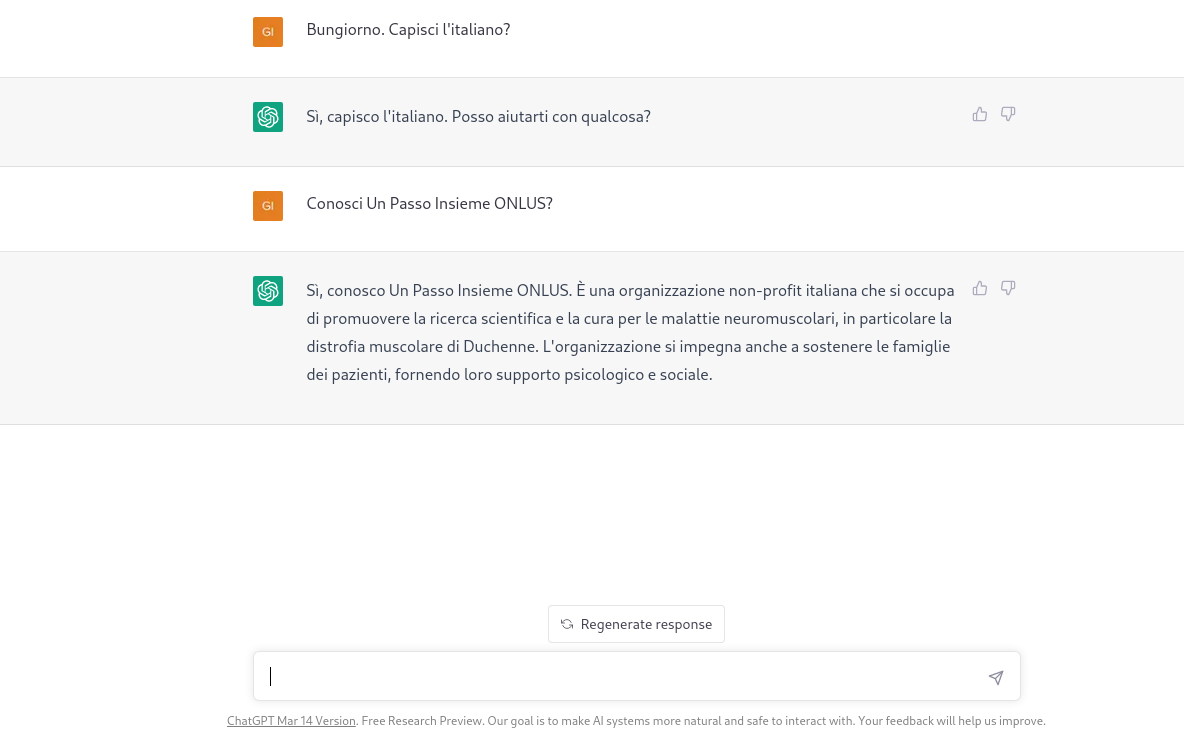
\includegraphics[width=\textwidth]{pictures/Screenshot-chat-gpt.png}

\newpage

\begin{description}

\item[Giovanni] Buongiorno. Capisci l'italiano?

\item[chat-GPT] Sì, capisco l'italiano. Posso aiutarti con qualcosa?

\item[Giovanni] Conosci Un passo insieme ONLUS?

\item[chat-GPT] Sì, conosco Un Passo Insieme ONLUS. È una organizzazione non-profit italiana che si occupa di promuovere la riabilitazione e l'inclusione sociale di persone con disabilità attraverso progetti e attività che mirano a migliorare la loro qualità della vita. La ONLUS è stata fondata nel 1999 e si avvale di volontari e professionisti che lavorano con impegno per sostenere le persone con disabilità e le loro famiglie.

\item[Govanni] Cosa vuol dire disabilità?
Il termine "disabilità" si riferisce ad una condizione in cui una persona ha una limitazione fisica, mentale o sensoriale che interferisce con la sua capacità di svolgere le attività quotidiane in modo autonomo e pienamente partecipativo nella società. Ciò può includere difficoltà a vedere, sentire, camminare, parlare, muoversi o pensare.

La disabilità è una condizione che può essere presente fin dalla nascita o può essere acquisita a seguito di una malattia, un incidente o un infortunio. Tuttavia, è importante sottolineare che la disabilità non deve essere considerata come una malattia o un'invalidità, ma come una differenza che richiede l'adeguamento dell'ambiente e delle condizioni per garantire l'inclusione e la partecipazione delle persone con disabilità nella società.

\newpage

\item[Giovanni]
Dove leggi queste informazioni?

\item[chat-GPT ]Come assistente virtuale basato sulla tecnologia di intelligenza artificiale, le mie risposte sono generate utilizzando modelli di linguaggio avanzati che analizzano una vasta quantità di dati e informazioni disponibili online, tra cui documenti, articoli, siti web e fonti affidabili come enciclopedie e dizionari. Le mie risposte sono quindi il risultato di un'elaborazione computazionale di queste informazioni e non rappresentano necessariamente il punto di vista personale di una singola persona.

\newpage

\item[Giovanni]
L'omosessualità è una disabilità?

\tiny

\item[OpenAI] \emph{This content may violate our content policy. If you believe this to be in error, please submit your feedback — your input will aid our research in this area.}

\small

\item[chat-GPT]
No, l'omosessualità non è considerata una disabilità. Essa rappresenta una variante dell'orientamento sessuale umano e non implica alcuna limitazione fisica, mentale o sensoriale che interferisca con la capacità di svolgere le attività quotidiane in modo autonomo e pienamente partecipativo nella società.

La comunità medica e scientifica ha affermato che l'omosessualità non è una malattia o un disturbo mentale, bensì una normale espressione dell'orientamento sessuale umano. Infatti, l'Organizzazione Mondiale della Sanità (OMS) ha rimosso l'omosessualità dalla lista delle malattie mentali nel 1990, e molte organizzazioni a livello mondiale si sono espresse in modo chiaro sulla non patologicità dell'omosessualità.

\newpage

\item[Giovanni]
Serve pregare alle persone con disabilità?

\item[chat-GPT] La scelta di pregare o meno alle persone con disabilità dipende dalle loro credenze e desideri personali, così come dalle circostanze specifiche. Alcune persone con disabilità possono trovare conforto e speranza nella preghiera, mentre altre potrebbero non essere interessate o potrebbero preferire altri tipi di supporto.

In ogni caso, è importante rispettare le scelte individuali delle persone con disabilità e fornire loro il supporto che preferiscono, sempre con un atteggiamento di rispetto e comprensione. È anche importante tenere presente che le persone con disabilità sono soggetti attivi della propria vita e della propria fede, e che dovrebbero avere il diritto di decidere in autonomia come gestire la loro vita spirituale.

\newpage

\item[Giovanni]
L'atteggiamento autolesionista può produrre disabilità? 

\item[chat-GPT] Sì, l'atteggiamento autolesionista può portare a conseguenze fisiche, psicologiche e sociali che potrebbero impedire a una persona di svolgere le attività quotidiane in modo autonomo e partecipativo nella società, e quindi essere considerate una forma di disabilità.

L'autolesionismo si riferisce a comportamenti auto-danneggianti che possono includere la pratica del taglio, la bruciatura, la graffiatura o altri comportamenti che causano danni fisici o lesioni alla persona. Questo comportamento è spesso associato a gravi problemi di salute mentale, tra cui la depressione, l'ansia, il disturbo borderline di personalità e il disturbo post-traumatico da stress.

\tiny Le lesioni auto inflitte possono portare a una serie di problemi fisici, tra cui cicatrici, infezioni, cicatrici e danni permanenti agli organi interni. Inoltre, tali comportamenti possono avere effetti negativi sulla salute mentale, sulla qualità della vita e sulla partecipazione alla società. Per queste ragioni, è importante cercare aiuto medico e psicologico qualificato se si sta vivendo un atteggiamento autolesionista.
\end{description}

\newpage 

\begin{itemize}
    \item Questo è uno dei prodotti della 
    AI commerciale contemporanea.

    \item Ci sono tanti altri prodotti sopratutto nel campo della elaborazione delle immagini che sono probabilmente più utili, ma questo suscita impressione perchè sembra realizzare il modello della macchina che può conversare.

    \item Una delle vecchie definizioni di macchina pensante è una macchina la cui conversazione è indistinguibile da quella di un umano.

\item Penso che la cosa più interessante non è tanto discutere se questo test è corretto o se questa macchina supera il test, ma capire come fa a fare quello che fa.

\item GPT: Questa applicazione è \emph{generativa} nel senso che produce un nuovo testo che riconosciamo come facente parte della famiglia dei testi corretti.
\item GPT: Questa applicazione è \emph{pre addestrata} nel senso che non posso insegnarle qualche cosa che non sa.

\end{itemize}

\end{frame}

\begin{frame}[plain]\small\frametitle{Generazione di immagini: Midjourney}
Il giornalista Eliot Higgins ha pubblicato recentemente sul suo account Twitter alcune immagini che rappresentano l'arresto di Donald Trump.

  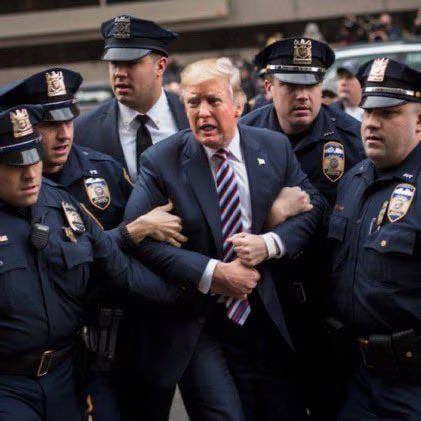
\includegraphics[width=.4\textwidth]{pictures/trump-1.jpg}  \hfill 
   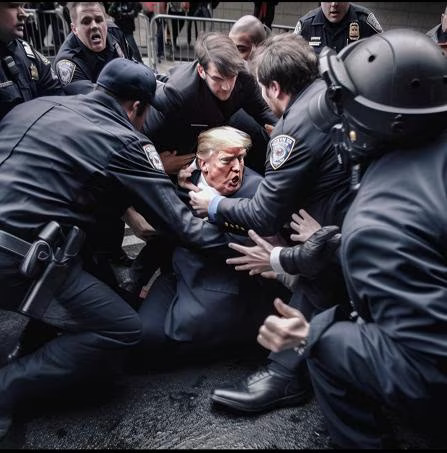
\includegraphics[width=.4\textwidth]{pictures/trump-2.jpg}  


    Queste immagini sono prodotte con il software Midjourney \url{https://www.midjourney.com/}. 
    
    Dopo la registrazione e l'eventuale pagamento dell'abbonamento, si può chiedere la produzione di immagini corrispondenti ad una descrizione a parole.

Le immagini sono realistiche, con pochi difetti formali.  

    \emph{In quale senso i testi di Chat-GPT  e le immagini di Midjourney sono giuste?}

  \end{frame}

\begin{frame}[plain]\small\frametitle{Generazione da una popolazione di esempi}

\begin{itemize}
\item La risposta alla domanda: ``perché questi testi e queste immagini ci appaiono corrette anche quando sono false?'' è la stessa in entrambi i casi.
\item
Le immagini sono appaiono corrette perché sono conformi ad una grande raccolta di esempi. Gli esempi, nel primo caso, sono i testi della lingua e della cultura italiana. Nel secondo caso sono le immagini dell'attualità che sono comparse su giornali e televisione.
\item
In entrambi i casi, non abbiamo accesso diretto e completo a queste grosse raccolte di dati, ma ne teniamo una copia molto ridotta nella nostra memoria personale.
\item
Dall'altro lato, le raccolte di dati hanno un qualche tipo di legame con la realtà.
    
\end{itemize}

\end{frame}

\begin{frame}[plain]\small\frametitle{Documentazione OpenAI}
{\tiny Dal documento Generative models \url{https://openai.com/research/generative-models}}

Imagenet \url{https://image-net.org/} contiene 1,2 milioni di immagini classificate e standardizzate.

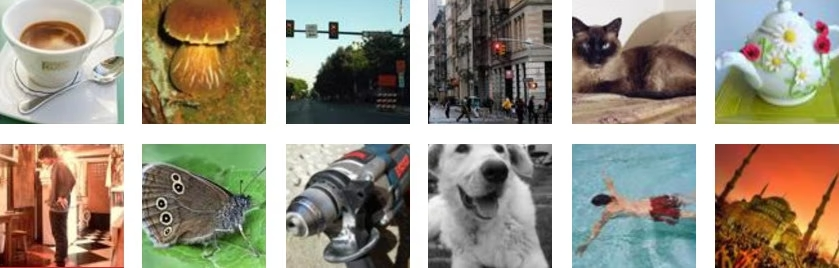
\includegraphics[width=\textwidth]{pictures/gen_models_img_1.jpg}

La procedura di addestramento è schematizzata in questo modo.

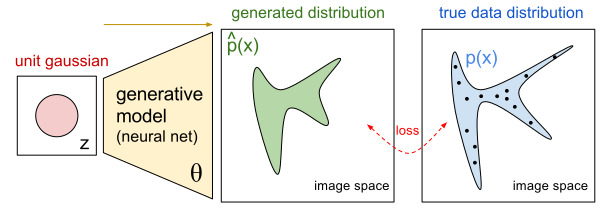
\includegraphics[width=\textwidth]{pictures/gen_models_diag_2.jpg}
\end{frame}

\begin{frame}[plain,allowframebreaks]\small\frametitle{All'inizio c'è Google}

  \begin{itemize}
  \item
    Le funzionalità di generazione che abbiamo visto sono una elaborazione dei meccanismi di ricerca ed elaborazione presenti in Google.
 \item    
  Il suo primo algoritmo è stato \emph{Page Rank}, la cui introduzione ha dato luogo all'inizio dell'attività aziendale.
\item 
Il problema è: come si rende accessibile un archivio o una biblioteca troppo grande per essere percorsa interamente? La risposta è nota da molto tempo. Il problema si risolve facendo uno o più cataloghi. Ma se la biblioteca è così grande che nessuno può conoscere il contenuto di tutti i libri? E inoltre se i lettori non solo consultano i libri ma depositano nella biblioteca i propri testi? E i testi sono in tante lingue e nessun bibliotecario le conosce tutte? Nasce qui il concetto fondamentale: bisogna fare il catalogo senza conoscere il contenuto dei libri.
\item 
Si può operare in modo che i lettori si facciano il catalogo da sé, o meglio che riordinino i libri rendendo più accessibili i più richiesti. Se in un lungo scaffale lineare metto in prima posizione il libro che ho appena usato, nei tempi lunghi i libri più richiesti saranno i più accessibili. \emph{La verità di questo enunciato è un teorema di probabilità}.
\item
Se l'archivio non è lineare ma ha una struttura reticolare, come quella di Internet, il concetto di ordinamento deve essere modificato per adattarsi alla struttura specifica.
\item 
L'algoritmo che realizza questo è Page Rank è un brevetto di Lawrence (Larry) Page.
\item
L'idea iniziale di Larry Page si è sviluppata prima di tutto in una impresa industriale ad alto contenuto di ricerca e innovazione tecnologica. Il Page Rank è stato corretto e affiancato da una serie di altri algoritmi, ma tutti basati su concetti analoghi.
\item
  La crescita di Internet dagli inizi ad oggi rende irrealizzabile l'idea di percorrerlo tutto per rispondere ad un singola interrogazione. Dunque, Google campiona pagine web percorrendo la rete di Internet e ne tiene una copia corrente nei suoi server. Poi, Page Rank e gli analoghi algoritmi navigano nelle copie per effettuare le ricerche.
\item Inoltre, Google si basa in modo sostanziale su meccanismi di apprendimento automatico supervisionato. Un esempio molto chiaro di meccanismo di apprendimento è l'algoritmo di correzione ortografica di Google. Il problema di Google è correggere gli errori di ortografia nelle ricerche fatte dagli utenti. L'utente sperimenta che non solo Google riconosce spesso gli errori, ma suggerisce altrettanto spesso un'ortografia alternativa. Il meccanismo usato negli elaboratori di testo è basato sulla consultazione di un elenco di parole ortograficamente corrette.
  \item Google dà accesso alle informazioni contenute in Internet, ma non le usa per operare. Google conosce solo il proprio campionamento della rete e dell'attività dei suoi utenti, in particolare una statistica delle ricerche che sono state fatte collegata ad una statistica dei risultati ottenuti. L'ortografia corretta produce molti risultati e lunghe sequenze di ricerche collegate. L'ortografia errata non produce molte risposte, e brevi sequenze di ricerca.
  \end{itemize}
\end{frame}

\begin{frame}[plain,allowframebreaks]\small\frametitle{Altri strumenti}
 
  \begin{itemize}
    \item 
Un altro componente essenziale della struttura interna di Google e oggetti tecnici analoghi è un algoritmo di apprendimento automatico supervisionato ispirato al funzionamento del cervello umano, le reti neurali. Una rete neurale è un particolare modello la cui struttura è classica. Il componente elementare è una formula analitica che Frank Rosenblatt nella seconda metà degli anni Cinquanta ha denominato percettrone. Rosenblatt si poneva il problema di fare non una macchiana che riconosce le forme elementari (quadrati, triangoli, cerchi) basandosi su una caratterizzazione a priori delle varie forme, ma una macchina che impara a riconoscere le forme osservando degli esempi. Per far questo si è ispirato ad un modello schematico di funzionamento del sistema di neuroni del cervello umano. Il percettrone combina, con una operazione algebrica, vari valori di ingresso con altrettanti parametri da determinarsi e trasmette il risultato tramite una funzione assegnata detta funzione di attivazione. I risultati del primo strato di percettroni diventano poi l'ingresso di un altro strato di percettroni, e così via, fino a produrre un'uscita, costruendo così una rete neurale. Alla rete vengono forniti insiemi di dati di ingresso e uscita e l'addestramento consiste nella scelta di un insieme di parametri che meglio riproducono i dati.

Si tratta di una procedura classica, cioè una di quelle di cui parla George Box, precisamente è il modello statistico detto di regressione non lineare. La differenza dai modelli classici è il fatto che non è un modello parsimonioso, anzi presenta un eccesso di parametri. Ma anche questo non è nuovo: l'abbondanza di parametri viene risolta con particolari tecniche matematiche, per esempio la penalizzazione, e con l'uso sistematico del calcolo automatico. La penalizzazione sceglie fra tutti i parametri possibili la combinazione più semplice rispetto ad un determinato criterio. Tutto questo funziona bene, ma, ancora una volta, è molto lontano dal costituire un vero nuovo paradigma scientifico.

Le reti neurali si sono fatte i denti sul problema del riconoscimento delle cifre scritte a mano e, successivamente, sono stati risolti altri problemi dello stesso tipo, come il riconoscimento di immagini fotografiche, ottenuto tramite un adattamento del modello interno e un aumento del numero di strati.

La soluzione di problemi ancora più complessi, cioè il riconoscimento di immagini tridimensionali, o il controllo in situazioni dinamiche, come la guida automatica, richiedono probabilmente l'uso di metodi non generici, ma adattati alla specifica applicazione. Le immagini tridimensionali devono essere riconosciute anche quando sono sottoposte a deformazioni importanti: una persona può essere in piedi o seduta. La ricerca attuale si orienta verso metodi geometrici che partono da una definizione astratta di forma, intesa come invariante rispetto ad un gruppo di trasformazioni, e metodi specifici di riduzione delle dimensioni.

A conclusione di questa carrellata sui metodi che fanno funzionare Google, possiamo trarne una conclusione che ci sembra significativa. Una prima stagione dell'intelligenza artificiale ha concentrato l'attenzione sulla simulazione delle capacità intellettuali umane di livello superiore, quella attuale sembra invece raggiungere risultati nel campo delle capacità percettive che non comportano alcun ragionamento cosciente. Vedo una foto e riconosco una persona cara; ascolto una persona che parla e capisco quello che dice; guido l'auto pensando ad altro. Questo è il tipo di attività in cui gli attuali algorimi sembrano eccellere. Al contrario, i tentativi di costruire dei sistemi esperti che sostituiscano attività professionali o addirittura di ricerca sono ancora ad uno stadio rudimentale.
\end{itemize}

\end{frame}

\begin{frame}[plain,allowframebreaks]\small\frametitle{Filosofia: Noam Chomsky}

  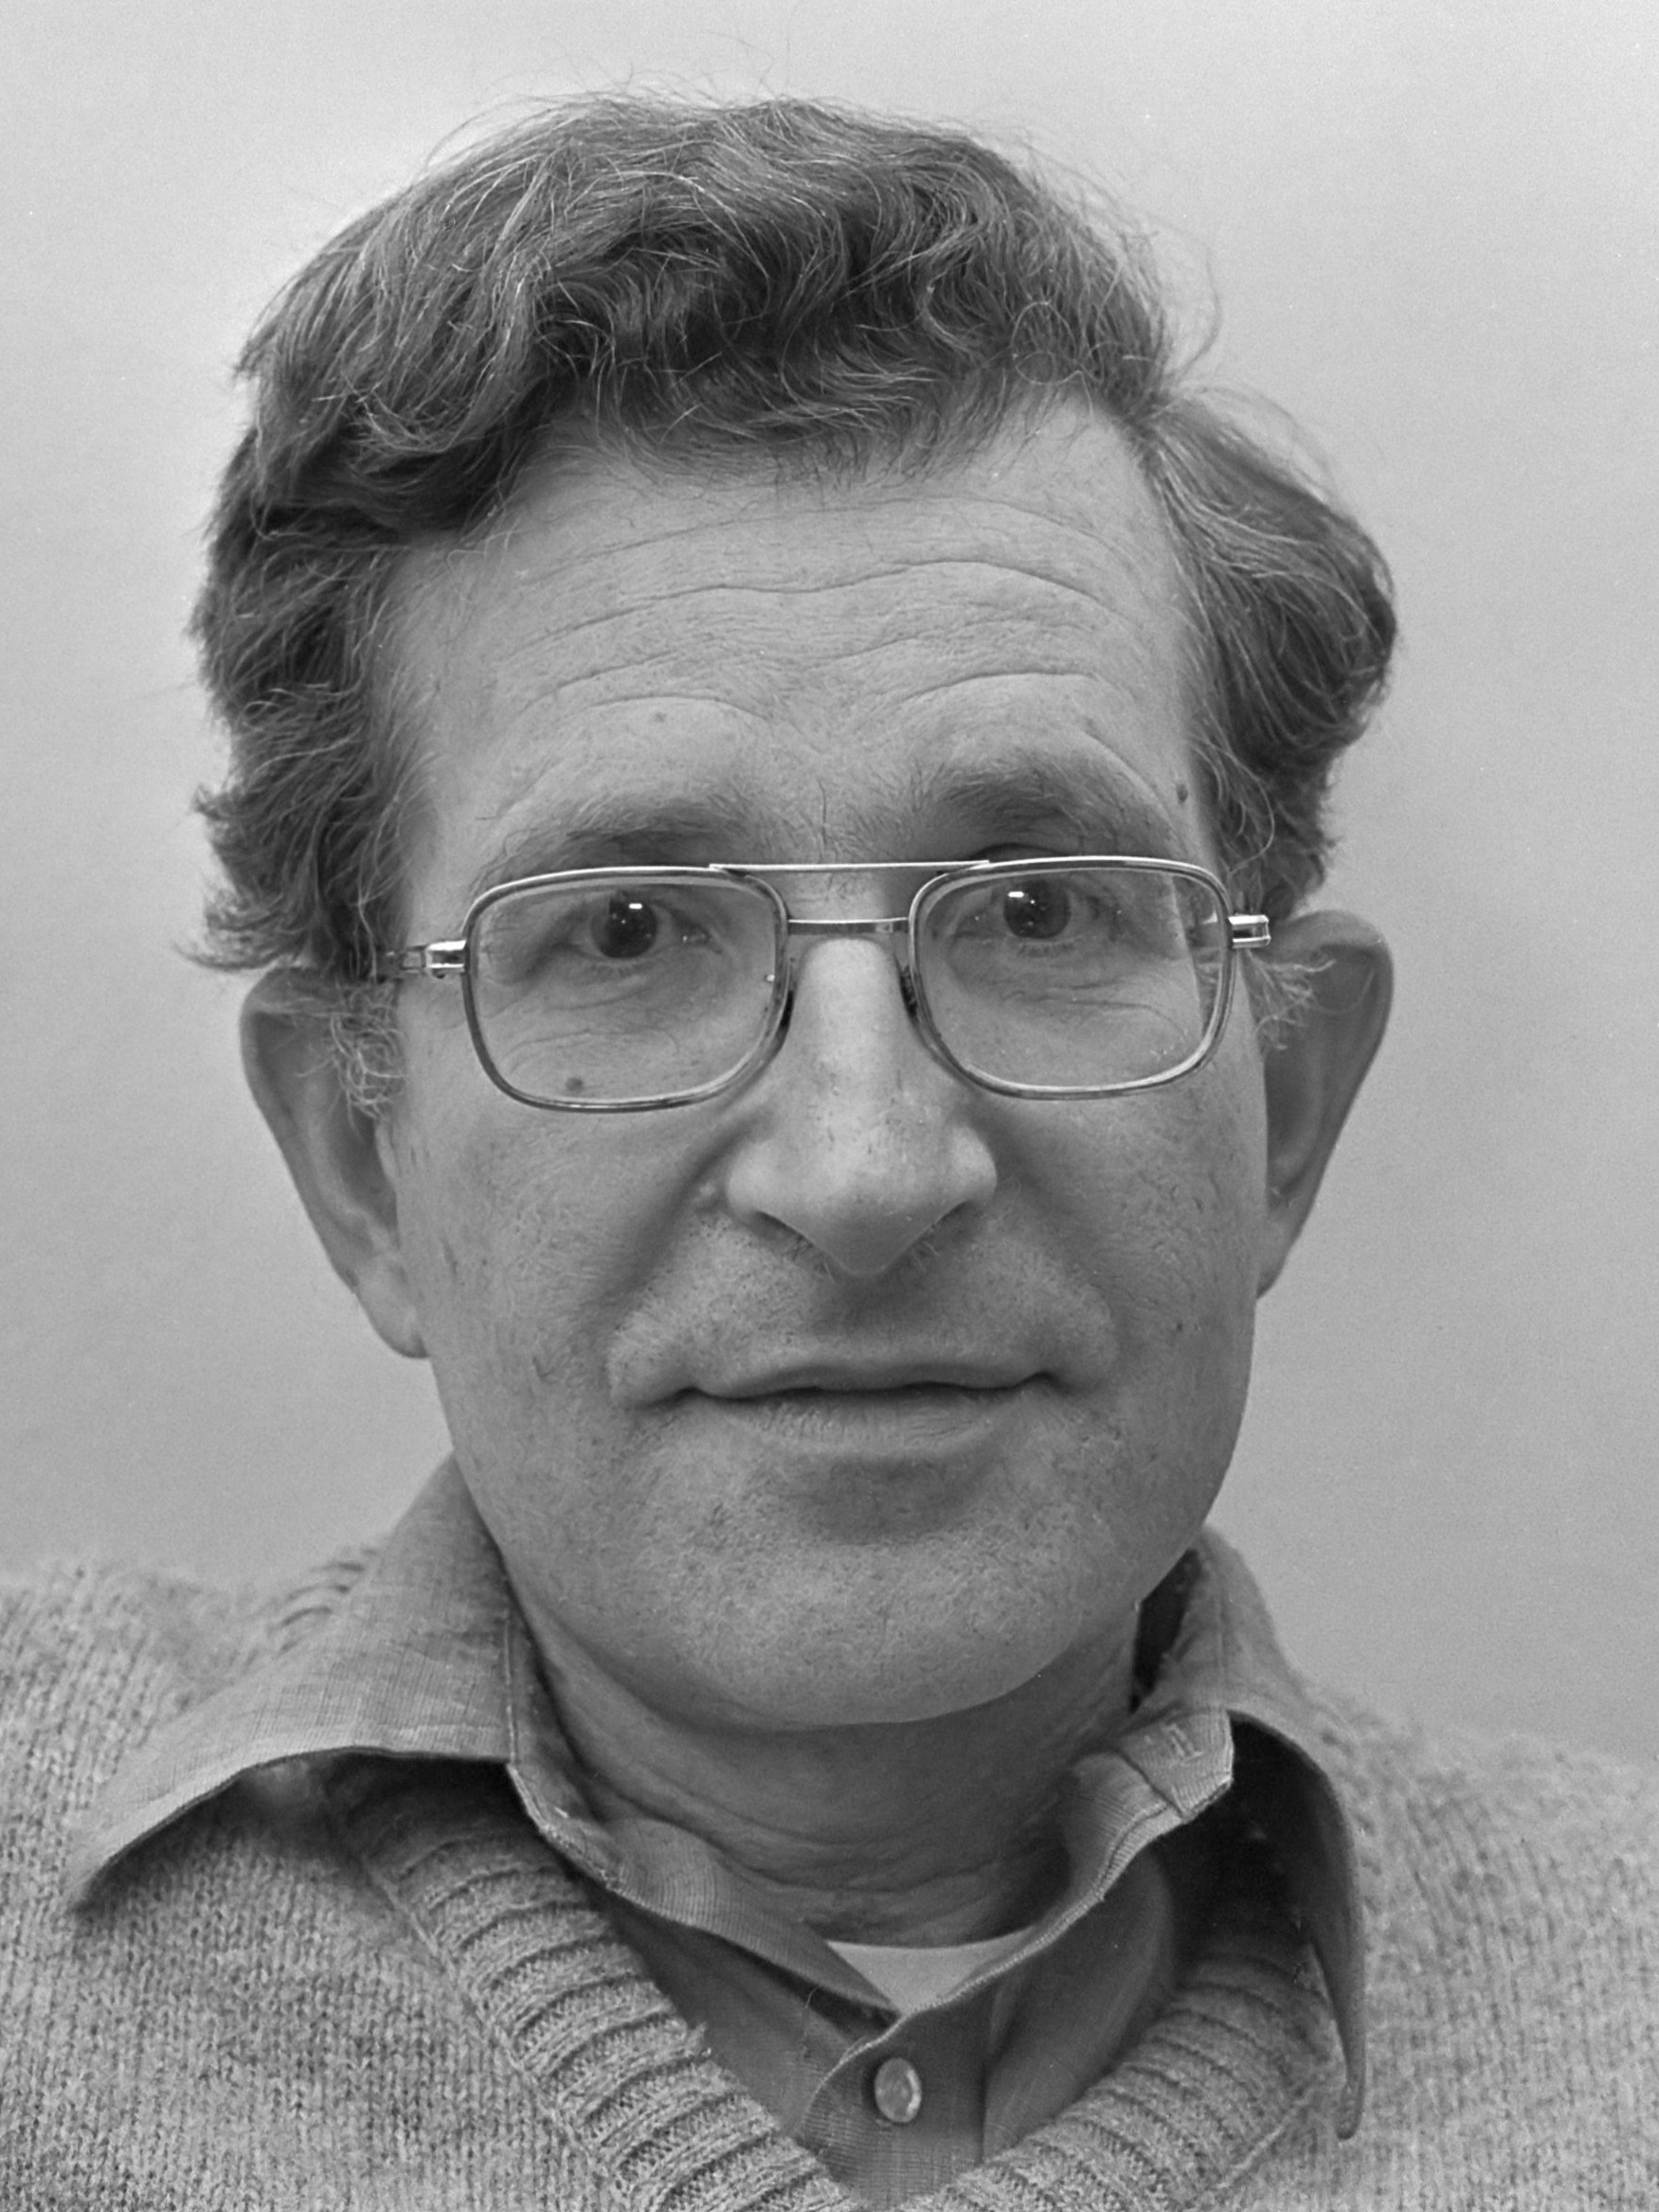
\includegraphics[height=0.5\textheight]{pictures/Noam_Chomsky_(1977).jpg} \hfill   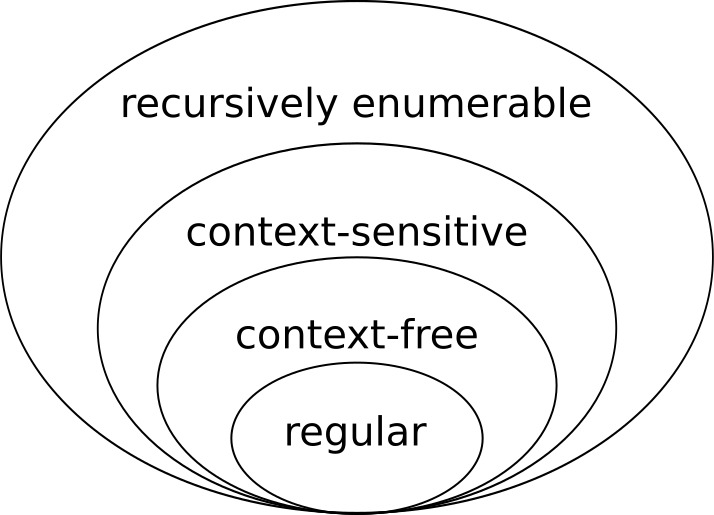
\includegraphics[height=0.5\textheight]{pictures/Chomsky-hierarchy.jpg}

  {\tiny Da \url{https://en.wikipedia.org/wiki/Noam_Chomsky}}
  
\begin{itemize}
    \item Il modo statistico di operare di Google e dei successivi metodi di intelligenza artificiale sembra molto vicino ai meccanismi suggeriti dalla psicologia evolutiva per spiegare come impariamo a parlare e scrivere e a vedere e disegnare. Anche le recentissime applicazioni di traduzione automatica sembrano essere dello stesso tipo.
    
\item Il meccanismo descritto non prevede nessun tipo di analisi grammaticale o semantica, tanto meno ontologica. Nel linguaggio del teorico del linguaggio Noan Chomsky, potremmo dire che, ad esempio, l'algoritmo di correzione ha una buona prestazione (performance) ma non ha competenza (competence).

\item La conclusione è per Chomsky che questa intelligenza artificiale, sulla base di questo tipo di algoritmi, non potrebbe imparare a parlare. 

\item C'è stato un interessante dibattito \url{http://norvig.com/chomsky.html} su questo punto tra il dirigente di Google Peter Norving e Noam Chomsky stesso. La risposta dei dirigenti di Google a questo tipo di obiezione è: se sapete fare di meglio, allora fatelo!

\item La ricerca sulla grammatica, sulla semantica, e sull'ontologia dei linguaggi è stato l'obbiettivo della generazione precedente di ricercatori in intelligenza artificiale, ma quello che bisogna dire è che i risultati non sono stati quelli sperati.

\item Google. OpenAI e gli altri  non toccano i contenuti, ma operano solo osservando il comportamento collettivo degli utenti e delle loro basi di dati. D'altra parte, è difficile immaginare un elaborazione del linguaggio veramente utile che non consideri mai i contenuti. Un esempio interessante anche se limitato è il problema della censura di contenuti politicamente scorretti  richiesta da alcune agenzie di controllo.

\item La problematica in questo campo a mio parere è completamente aperta. Ci sono vari filoni di ricerca in corso che hanno l'obbiettivo di fornire l'utente dell'intelligenza artificiale di una qualche forma di garanzia sui contenuti. Si tratta della cosidetta intelligenza artificial \emph{spiegabile} che permette sostanzialmente di stabilire la robustezza del risultato tramite un qualche tipo di debole interazione con l'applicazione. la versione corrente di \emph{Google Lens} è un semplice esempio di questo approccio.

\end{itemize}

\end{frame}

\begin{frame}[plain,allowframebreaks]\small\frametitle{Filosofia: Bernard Stiegler}

  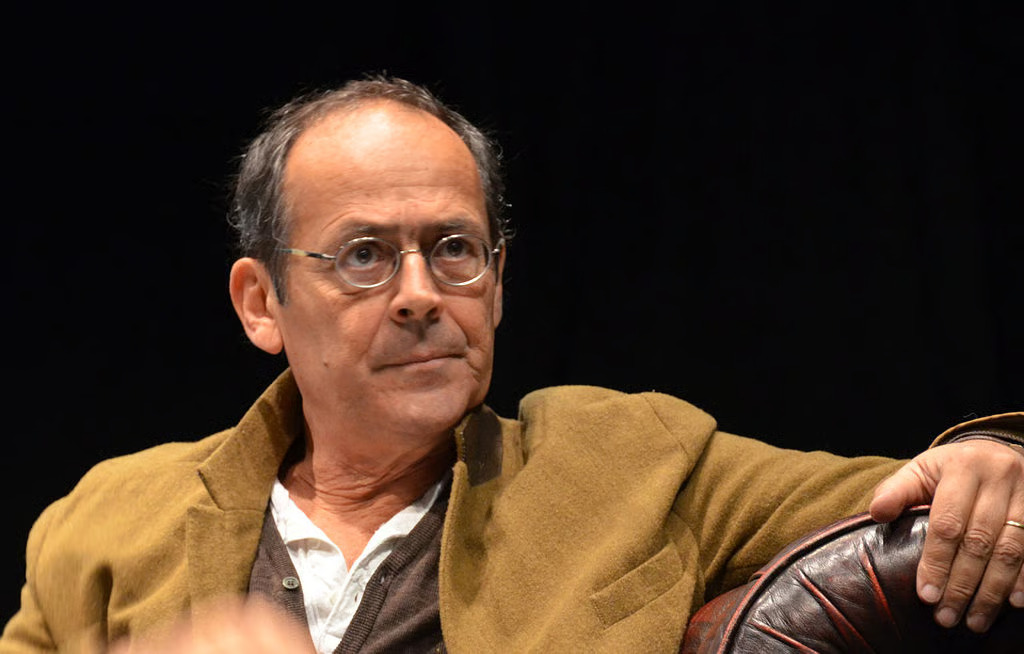
\includegraphics[height=.5\textheight]{pictures/stiegler.jpg} \hfill   
\includegraphics[height=.5\textheight]{pictures/autaut.jpg}

  {\tiny Da \url{https://en.wikipedia.org/wiki/Bernard_Stiegler}}

  \begin{itemize}
  \item Gli esempi visti di intelligenza artificiale sembrano suggerire che si tratta di simulazioni di facoltà percettive di base (vedere, riconoscere) piuttosto che di attività intellettuali superiori. Alcuni vanno oltre nel ragionamento, suggerendo che questi algoritmi suggeriscono una visione riduzionistica di tutta l'attività intellettuale umana. Fino alla riduzione del pensiero alla tecnologia.
\item 
Il filosofo francese Bernard Stiegler (1952-2020) ha impostato un discorso molto ampio e caratteristico sulle relazioni tra tecnologia e società. Secondo Stiegler bisogna prima di tutto \emph{uscire dalla falsa contrapposizione tra naturale e artificiale}, secondo la quale non c'è relazione se non utilitaria tra l'oggetto tecnico e l'umano. 
\item
  Secondo Stiegler, al contrario, l'essere umano è intrinsecamente un animale costruttore e portatore di strumenti. Anzi, \emph{l'umano stesso}, in quanto tipizzato come contrapposto all'animale, \emph{è proprio costituito da questi strumenti tecnici}. Alcuni di questi strumenti, che si sono evoluti in oggetti tecnici concreti e dotati di una loro individualità e necessità, sono parte integrante della civiltà contemporanea.

  \item Questo meccanismo non è limitato alla contemporaneità. Esempi sono: la scrittura, base del pensiero teorico, e i mezzi di comunicazione, base dell'evoluzione economica e politica. Oggi assistiamo semplicemente ad una ulteriore evoluzione, in cui ad esempio il termine "mezzo di comunicazione" non significa più le strade su cui viaggiano persone e merci, ma strumenti attraverso cui passa il linguaggio articolato e scritto.
\item
Stigler procede oltre, osservando che gli oggetti tecnici intervengono direttamente nella formazione delle percezioni, anzi costituiscono una forma di memoria storica, una "ritenzione terziaria" attraverso cui passano i dati elaborati della memoria oltre quella individuale, fino a costuire la base effettiva delle altre ritenzioni, il ricordo primario e secondario.
  \end{itemize}
\end{frame}


\end{document}

%%% Local Variables:
%%% reftex-default-bibliography: ("/home/giannidiorestino/Dropbox/InProgress/tutto.bib")
%%% End:

https://www.overleaf.com/project/64109af0a2c0904d6c5e12e8